\documentclass{book}
\usepackage{commeunjeustyle}
%%%%%%%%%%%%%%%%%%%%%%%%%%%%
\begin{document}
\chapter*{Endomorphismes remarquables d'un espace euclidien}

Dans un espace euclidien $E$, l'objectif est  d'étudier les transformations de $E$ qui préservent le produit scalaire. Ainsi on cherche à remplacer
les notions de base, équation linéaire, forme linéaire, transposition etc. par les notions
pertinentes en géométrie euclidienne à savoir, respectivement, de base orthonormée,
de vecteurs normaux, de produit scalaire etc.\\
Les applications de ces transformations sont multiples :
\begin{itemize}
\item  résoudre des équations différentielles linéaires,  trouver une base orthogonale pour deux formes quadratiques si l'une est définie positive ou de classifier les quadriques,
\item en physique,  résoudre de nombreuses équations aux dérivées partielles comme celle de la corde vibrante ou exprimer le moment d'inertie d'un solide,
\item en apprentissage automatique, calibrer un modèle de régression à l'aide de la méthode des moindres carrés ou étudier un échantillon en réduisant la dimension à l'aide de l'analyse en composantes principales.
\end{itemize} 
Dans ce chapitre, $(E,\PS{}{})$ désigne un espace euclidien de dimension $n\in \N^*$. 
\section{Isométrie vectorielle et matrice orthogonale}
\subsection{Isométrie vectorielle}
\begin{Definition}[Isométrie vectorielle]
On appelle \defi{isométrie vectorielle ou automorphisme orthogonal de E} tout endomorphisme préservant le produit scalaire, i.e. si
$$ \forall \vec{x},\vec{y}\in E:\quad \PS{u(\vec{x})}{ u(\vec{y})} =\PS{\vec{x}}{\vec{y}}. $$ 
On appelle \defi{groupe orthogonal} l'ensemble de ces endomorphismes et on le note
\defi{$\OrE$}.
\end{Definition}
\begin{Proposition}[Conservation de la norme]
$u$ est une isométrie vectorielle si et seulement si 
$$ \forall \vec{x}\in E:\quad \norme{u(\vec{x})} =\norme{\vec{x}}. $$ 
\end{Proposition}
\begin{Demonstration}
\begin{itemize}
\item \textit{Implication :} Soit $\vec{x}\in E$.  En prenant  $\vec{x}= \vec{y}$, on obtient $\PS{u(\vec{x})}{ u(\vec{x})} =\PS{\vec{x}}{\vec{x}}$, soit $\norme{u(\vec{x})}^2 =\norme{\vec{x}}^2$, d'où $\norme{u(\vec{x})} =\norme{\vec{x}}.$
\item \textit{Réciproque :} Soit $\vec{x},\vec{y}\in E$. On a 
$$\begin{aligned}
\PS{u(\vec{x})}{ u(\vec{y})}\overbrace{=}^{\text{Identité de polarisation}}&\frac{1}{4}(\norme{u(\vec{x})+u(\vec{y})}-\norme{u(\vec{x})+u(\vec{y})} )\\
\overbrace{=}^{\text{Linéarité}}&\frac{1}{4}(\norme{u(\vec{x}+\vec{y})}-\norme{u(\vec{x}-\vec{y})} )\\
\overbrace{=}^{\text{Conservation de la norme}}&\frac{1}{4}(\norme{\vec{x}+\vec{y}}-\norme{\vec{x}-\vec{y}} )\\
\overbrace{=}^{\text{Identité de polarisation}}&\PS{\vec{x}}{ \vec{y}}
\end{aligned}$$
\end{itemize}
\end{Demonstration}
\begin{Proposition}[Conservation d'une base orthonormale]
$u$ est une isométrie vectorielle si et seulement si l'image d'une base orthonormale quelconque est une base orthonormale.
\end{Proposition}
\begin{Demonstration}
\begin{itemize}
\item \textit{$ \Rightarrow$ :} Soit $(\vec{e_1},\dots,\vec{e_n})$ une base orthonormale de $E$. Comme
$$\PS{u(\vec{e_i})}{ u(\vec{e}_j)}\overbrace{=}^{\text{Conservation du produit scalaire}}\PS{\vec{e_i}}{ \vec{e_j}}\overbrace{=}^{(\vec{e_1},\dots,\vec{e_n}) \text{BON}}\begin{cases}1&\text{si }i=j\\0&\text{si }i\neq j\end{cases},$$ $(u(\vec{e_1}),\dots,u(\vec{e_n}))$ est bien une base orthonormale de $E$. 
\item \textit{$ \Leftarrow$ :} Soit $(\vec{e_1},\dots,\vec{e_n})$ une base orthonormale de $E$ tel que $(u(\vec{e_1}),\dots,u(\vec{e_n}))$ est aussi une base orthonormale de $E$. \\
Soit $\vec{x}=\sum_{i=1}^n x_i\vec{e_i},\vec{y}=\sum_{i=1}^n y_i\vec{e_i}\in E$. On a 
$$\begin{aligned}
\PS{u(\vec{x})}{ u(\vec{y})}=&\PS{u\left(\sum_{i=1}^n x_i\vec{e_i}\right)}{u\left(\sum_{j=1}^n y_j\vec{e_j}\right)}\\
\overbrace{=}^{\text{bilinéarité}}& \sum_{i=1}^n \sum_{j=1}^n x_i y_j \PS{u(\vec{e_i})}{u(\vec{e_j})}\\
=& \sum_{i=1}^n \sum_{j=1}^n x_i y_j \PS{\vec{e_i})}{u(\vec{e_j}}\text{ car }\quad \PS{u(\vec{e_i})}{u(\vec{e_j})}\overbrace{=}^{BON}\begin{cases}1&\text{si }i=j\\0&\text{si }i\neq j\end{cases}\overbrace{=}^{BON}\PS{\vec{e_i}}{\vec{e_j}}\\
\overbrace{=}^{\text{bilinéarité}}&\PS{\sum_{i=1}^n x_i\vec{e_i}}{\sum_{j=1}^n y_j\vec{e_j}}\\
=&\PS{\vec{x}}{ \vec{y}}\\
\end{aligned}$$
\end{itemize}
\end{Demonstration}
\begin{Proposition}[Groupe]
$\OrE$ est un groupe, sous groupe de $\GLE$.
\end{Proposition}
\begin{Demonstration}
$\OrE$ est un sous groupe de $\GLE$.
\begin{itemize}
\item \textit{$\OrE\subset \GLE$} Soit $u\in \OrE$ Comme $u$ est un endomorphisme en dimension finie, il suffit de montrer que $u$ est injective, $\Ker u=\{\vec{0_E}\}$.\\
Soit $\vec{x}\in  \Ker u$. On a $u( \vec{x})=0$, d'où $\norme{u(\vec{x})}=\norme{\vec{0}}=0$.   Comme $\norme{u( \vec{x})}\overbrace{=}^{u\in\OrE }\norme{\vec{x}}$, on a $\norme{\vec{x}}=0$. Enfin $\vec{x}=\vec{0_E}$ car une norme est définie.
\item \textit{Non vide :} $Id_E\in \OrE$
\item \textit{Stabilité composition :} Soit $u,v \in \OrE$. Soit $\vec{x}\in  E$. La norme est conservée car :
$$ \norme{u(v(\vec{x}))}\overbrace{=}^{u\in \OrE}\norme{v(\vec{x})}\overbrace{=}^{v\in \OrE}\norme{\vec{x}}.$$
\item \textit{Stabilité inversion :} Soit $u \in \OrE$. Comme $u$ est un automorphisme, $u^{-1}$ l'est aussi. De plus, la norme est conservée car : 
$$ \norme{\vec{x}} = \norme{u( u^{-1}(\vec{x}))}\overbrace{=}^{u\in\OrE }\norme{u^{-1}(\vec{x})}.$$
\end{itemize}
\end{Demonstration}
\subsection{Matrice orthogonale}
\begin{Definition}[Matrice orthogonale]
Une matrice carrée $M \in \Mn{n}{R}$ est dit \defi{orthogonal} si $$\transposee{M} M = I_n.$$
On note \defi{$\OnR$} l'ensemble des matrices orthogonales de taille $n$.\\
Comme $\transposee{M} M = I_n$, la matrice $M$ est inversible d'inverse $\transposee{M}$ et on a aussi $ M \transposee{M}= I_n.$
\end{Definition}

\begin{Exemple} Dans $\R^2$, la matrice de rotation plane d'angle $\theta  $ :
$${\begin{pmatrix}\cos \theta &-\sin \theta \\\sin \theta &\cos \theta \end{pmatrix}}$$
ou dans $\R^3$, la matrice de rotation autour de  l'axe $\vec{e_1}=(1,0,0)$ et d'angle $\theta  $ ,
$$
 R_{\vec{e_1}}(\theta )={\begin{pmatrix}1&0&0\\0&\cos \theta &-\sin \theta \\0&\sin \theta &\cos \theta \end{pmatrix}}$$
ou les matrices de permutation, comme
$$
{\displaystyle {\begin{pmatrix}0&1&0\\0&0&1\\1&0&0\end{pmatrix}}.}$$
\end{Exemple}
\begin{Proposition}
$O \in \OnR$ si et seulement si la famille des colonnes de $O$ (ou les lignes) est une base orthonormale de l'espace euclidien canonique $\R^n$.
\end{Proposition}
\begin{Demonstration}
Soit $C_1,\dots,C_n$ les colonnes de la matrice $O$.
$$\begin{aligned}
O \in \OnR\text{  est  orthogonal } \Leftrightarrow&  \transposee{M} M =\begin{pmatrix}
\transposee{C_1}\\\vdots\\\transposee{C_n}
\end{pmatrix} \begin{pmatrix}
C_1&\dots&C_n
\end{pmatrix}=\begin{pmatrix}
\transposee{C_1}C_1 &\dots&\transposee{C_1}C_n\\
\vdots &&\vdots\\
\transposee{C_n}C_1&\dots&\transposee{C_n}C_n\\
\end{pmatrix} =  I_n\\
 \Leftrightarrow& \forall i,j\in\Intf{1}{n} :\quad \transposee{C_i}C_j=\delta_{ij}\\
\Leftrightarrow& \forall i,j\in\Intf{1}{n} :\quad \PS{C_i}{C_j}=\delta_{ij}\\
\Leftrightarrow& (C_1,\dots,C_n)\text{ est une base orthonormale de l'espace euclidien canonique } \R^n
\end{aligned}$$ 
Du fait de l'égalité $ O\transposee{O}=I_n$, on a le même résultat sur les lignes.
\end{Demonstration} 
\begin{Exemple}
Il est facile de vérifier qu'une matrice de permutation est une matrice orthogonal car ses vecteurs colonnes forment une famille orthonormale. 
\end{Exemple}

\begin{Theoreme}[Isométrie vectorielle et matrice orthogonale]
Soit $u\in\LE$. Soit $\mathcal{B}$ une base orthonormale de $E$.\\
$u$ est une isométrie vectorielle si et seulement si $[u]_\mathcal{B}$ est une matrice orthogonale.
\end{Theoreme}
\begin{Demonstration}
Soit $\mathcal{B}=(\vec{e_1},\dots,\vec{e_n})$ une base orthonormale de $E$.\\
Soit $C_1,\dots,C_n$ les colonnes de la matrice $[u]_\mathcal{B}$. On a  $[u(\vec{e_i})]_{\mathcal{B}}=C_i$.\\
Le coefficient de la matrice $\transposee{[u]_{\mathcal{B}}}[u]_{\mathcal{B}} $ d'indice $i,j$ est :\\
$$\transposee{C_i}C_j\overbrace{=}^{\mathcal{B} \text{ BON}}\PS{u(\vec{e_i})}{u(\vec{e_j})}.$$
\begin{itemize}
\item Si $u\in\OrE$, alors $\PS{u(\vec{e_i})}{u(\vec{e_j})}\overbrace{=}^{\text{Conservation d'une base orthonormale}}\delta_{ij}$ et donc $\transposee{[u]_{\mathcal{B}}}[u]_{\mathcal{B}} =I_n$, d'où $[u]_{\mathcal{B}}\in \OnR.$
\item Si $[u]_\mathcal{B}\in\OnR$, alors $\transposee{C_i}C_j=\delta_{i,j}$, soit $\PS{u(\vec{e_i})}{u(\vec{e_j})}=\delta_{ij}$ c'est à dire que l'image d'une base orthonormale et une  base orthonormale donc  $u\in\OrE.$
\end{itemize}
\end{Demonstration}
\begin{Proposition}[Matrice de passage d'un changement de bases orthonormales]
Soit $\mathcal{B},\mathcal{B}'$ deux bases orthonormales de $E$.\\
Alors la matrice de passage de base $\mathcal{B}$ à la base $\mathcal{B}'$, $P_{\mathcal{B}\to\mathcal{B}'}$, est une matrice orthogonale. 
Ainsi, son inverse est $P_{\mathcal{B}'\to\mathcal{B}}=  P^{-1}_{\mathcal{B}\to\mathcal{B}'}=\transposee{P_{\mathcal{B}\to\mathcal{B}'}}.$
\end{Proposition}
\begin{Demonstration}
Soit $u$ l'endomorphisme associée à la matrice de passage. Comme l'image d'une base orthonormale est une base orthonormale $f(\mathcal{B})=\mathcal{B}'$,  $f$ est une isométrie vectoriel, donc  $P_{\mathcal{B}\to\mathcal{B}'}$ est une matrice orthogonale.
\end{Demonstration}
\begin{Proposition}[Groupe]
$\OnR$ est un groupe, sous groupe de $\GLn{\R}$.
\end{Proposition}
\begin{Demonstration}
Pour la démonstration, il suffit de se ramener à $u$ l'endomorphisme associée à la matrice orthogonale qui est une isométrie vectorielle.
\end{Demonstration}
\subsection{Déterminant}

\begin{Proposition}[Déterminant]
Soit $O\in \OnR$.\\
Alors $ \det O= \pm 1$.\\
 Soit $u\in \OrE$.\\
Alors $ \det u= \pm 1$.
\end{Proposition}
\begin{Demonstration}
Comme $\transposee{O}O=I_n$, on a $\det (\transposee{O}O) =\det(I_n)=1$. Or $det (\transposee{O}O)=det \transposee{O}\det O=(\det O)^2$. Donc $ \det O= \pm 1$. \\
Soit $\mathcal{B}$ une base orthonormée de $E$.  Comme $[u]_{\mathcal{B}}\in \OnR$ et $\det u= \det [u]_{\mathcal{B}}$, on conclut que $ \det u= \pm 1$.
\end{Demonstration}
\begin{Remarque}
Une matrice ou un endomorphisme de déterminant 1 ou -1 n'est pas nécessairement une matrice orthogonale ou une isométrie vectorielle. Par exemple $\det \begin{pmatrix}1 &1\\0&1\end{pmatrix}=1$, mais les colonnes ne forment pas une base orthonormale de $\R^2$. Donc $\begin{pmatrix}1 &1\\0&1\end{pmatrix}\notin\mathcal{O}_2(\R)$. 
\end{Remarque}
\begin{Definition}[Rotation et groupe spéciale orthogonale]
Une matrice orthogonale [resp. isométrie] est \defi{direct(e)} si son déterminant est 1, indirect(e) si son déterminant est -1.\\
Une isométrie vectorielle directe est également appelée \defi{rotation}.\\
On note $\SOnR$ l'ensemble des matrices orthogonales directes de $\Mn{n}{\R}$ et $\SOE$ l'ensemble des rotations de $E$.
\end{Definition}
\begin{Exemple}
$\begin{pmatrix}0 &1\\-1&0\end{pmatrix}\in \mathcal{SO}_2(\R)$.
\end{Exemple}
\begin{Proposition}[Groupe]
$\SOnR$ [resp. $\SOE$ ] est un groupe, sous-groupe de $\OnR$ [resp. $\OrE$)] appelé \defi{groupe
spécial orthogonal} de $\Mn{n}{\R}$ [resp. $E$].
\end{Proposition}
\begin{Demonstration}
\begin{itemize}
\item \textit{Non vide} : $I_n\in \SOnR$.
\item \textit{Stabilité} :  Soit $S_1,S_2\in \SOnR$. $$\det (S_1 S_2^{-1})=\det S_1 \det S_2^{-1}=\frac{\det S_1}{ \det S_2}=1.$$
\end{itemize}
\end{Demonstration}
\subsection{Symétrie orthogonale}
\begin{Definition}[Symétrie orthogonale]
On appelle \defi{symétrie orthogonale} par rapport à $F$ parallèlement à $F^{\perp}$.\\
Si $F$ est un hyperplan de $E$, on parle alors de \defi{réflexion}.
\end{Definition}
%TODO SCHEMA EXEMPLE
\begin{Proposition}[Symétrie orthogonale]
Soit $u$ une isométrie vectorielle.\\
$u$ est une symétrie orthonormale si et seulement si sa matrice dans une base orthonormale est symétrique.  
\end{Proposition}
\begin{Demonstration}

\begin{itemize}
\item $\Longrightarrow :$ Soit une symétrie orthonormale par rapport à $F$ et $F^{\perp}$. Soit $\mathcal{B}$ une base orthonormale adaptée à décomposition  $F\oplus F^{\perp}=E.$ La matrice de $u$ dans la base $\mathcal{B}$ est de la forme :
$$[u]_\mathcal{B}= \begin{pmatrix}\mathrm {I}_{\dim(F_1)}&\mathrm {0}\\\mathrm {0} & -\mathrm {I}_{\dim(F_2)}\end{pmatrix}$$
Elle est symétrique. Soit $\mathcal{B}'$ une base orthonormale quelconque. La matrice de passage de BON $\mathcal{B}$ à la base BON $\mathcal{B}'$ est orthogonale donc $P^{-1}_{\mathcal{B}\to\mathcal{B}' }=\transposee{P_{\mathcal{B}\to\mathcal{B}'}}$. On a : 
$$[u]_{\mathcal{B}'}= \transposee{P_{\mathcal{B}\to\mathcal{B}'}} \begin{pmatrix}\mathrm {I}_{\dim(F_1)}&\mathrm {0}\\\mathrm {0} & -\mathrm {I}_{\dim(F_2)}\end{pmatrix}P_{\mathcal{B}\to\mathcal{B}'}$$
Donc $[u]_{\mathcal{B}'}$ est symétrique.
\item $\Longleftarrow :$ Voir théorème spectral.
\end{itemize}
\end{Demonstration}

\subsection{Orientation}
\begin{Definition}[Orientation]
Deux bases $\mathcal{B}$ et $\mathcal{B}'$ de $E$ ont même \defi{orientation} si $\det_\mathcal{B}(\mathcal{B}') > 0.$\\
Orienter $E$, c'est choisir une base $\mathcal{B}$ de référence. Une base $\mathcal{B}'$ est directe si elle a la même
orientation que $\mathcal{B}$.
\end{Definition}
\begin{Exemple}
Sur $\R^2$. La base de référence est $(\vec{e_1},\vec{e_2})$ la base canonique. Soit  $\mathcal{B}'=(-\vec{e_1},\vec{e_2}).$ Comme $\det_\mathcal{B}(\mathcal{B}')=\det \begin{pmatrix}-1&0\\0&1
\end{pmatrix}=-1$, $\mathcal{B}'$ est une base indirecte.
\end{Exemple}
\begin{Proposition}
Soit $\mathcal{B}$ une base orthonormée directe.\\
$\mathcal{B}'$ est une base orthonormée directe si seulement si la matrice de passage de $\mathcal{B}$ à $\mathcal{B}'$ est orthogonale directe.
\end{Proposition}
\begin{Demonstration}
L'équivalence est due à l'égalité :
$$ \det_\mathcal{B}(\mathcal{B}')=\det( P_{\mathcal{B}\to\mathcal{B}'})$$
\end{Demonstration}
\begin{Definition}[Orientation d'un hyperplan]
Orienter l'hyperplan $H$, c'est choisir un vecteur $\vec{n}$ orthogonal à $H$.\\
Une base $(\vec{e_1},...,\vec{e_{n-1}})$
de $H$ est alors directe si la base $(\vec{u},\vec{e_1},...,\vec{e_{n-1}})$ est directe dans $E$.\\
Il y a deux orientations possibles de H.
\end{Definition}
\begin{Exemple}
Soit $\R^3$ orientée par rapport à la base canonique. Soit $H$ l'hyperplan définie par le vecteur normale $(1,1,1)$. La base $((1,-1,0),(1,0,-1)$ de $H$ est directe car $\det \begin{pmatrix}1&1&1\\1&-1&0
\\1&0&-1\end{pmatrix}=3$. 
\end{Exemple}


\subsection{Isométrie vectorielle du plan}
\begin{Proposition}[Classification]
Les matrices de $\mathcal{O}_2(\R)$ sont les matrices de la forme :
$$ R_\theta = \begin{pmatrix} \cos \theta &-\sin \theta \\ \sin \theta & \cos \theta \end{pmatrix}; S_{\theta}=\begin{pmatrix} \cos \theta &\sin \theta \\ \sin \theta & -\cos \theta \end{pmatrix} \text{ où } \theta \in \R.$$
Les matrices de $\mathcal{SO}_2(\R)$ sont les $R_\theta$, $\theta \in \R$.\\
Les matrices indirectes sont les $S_\theta$, $\theta \in \R$.
\begin{center}
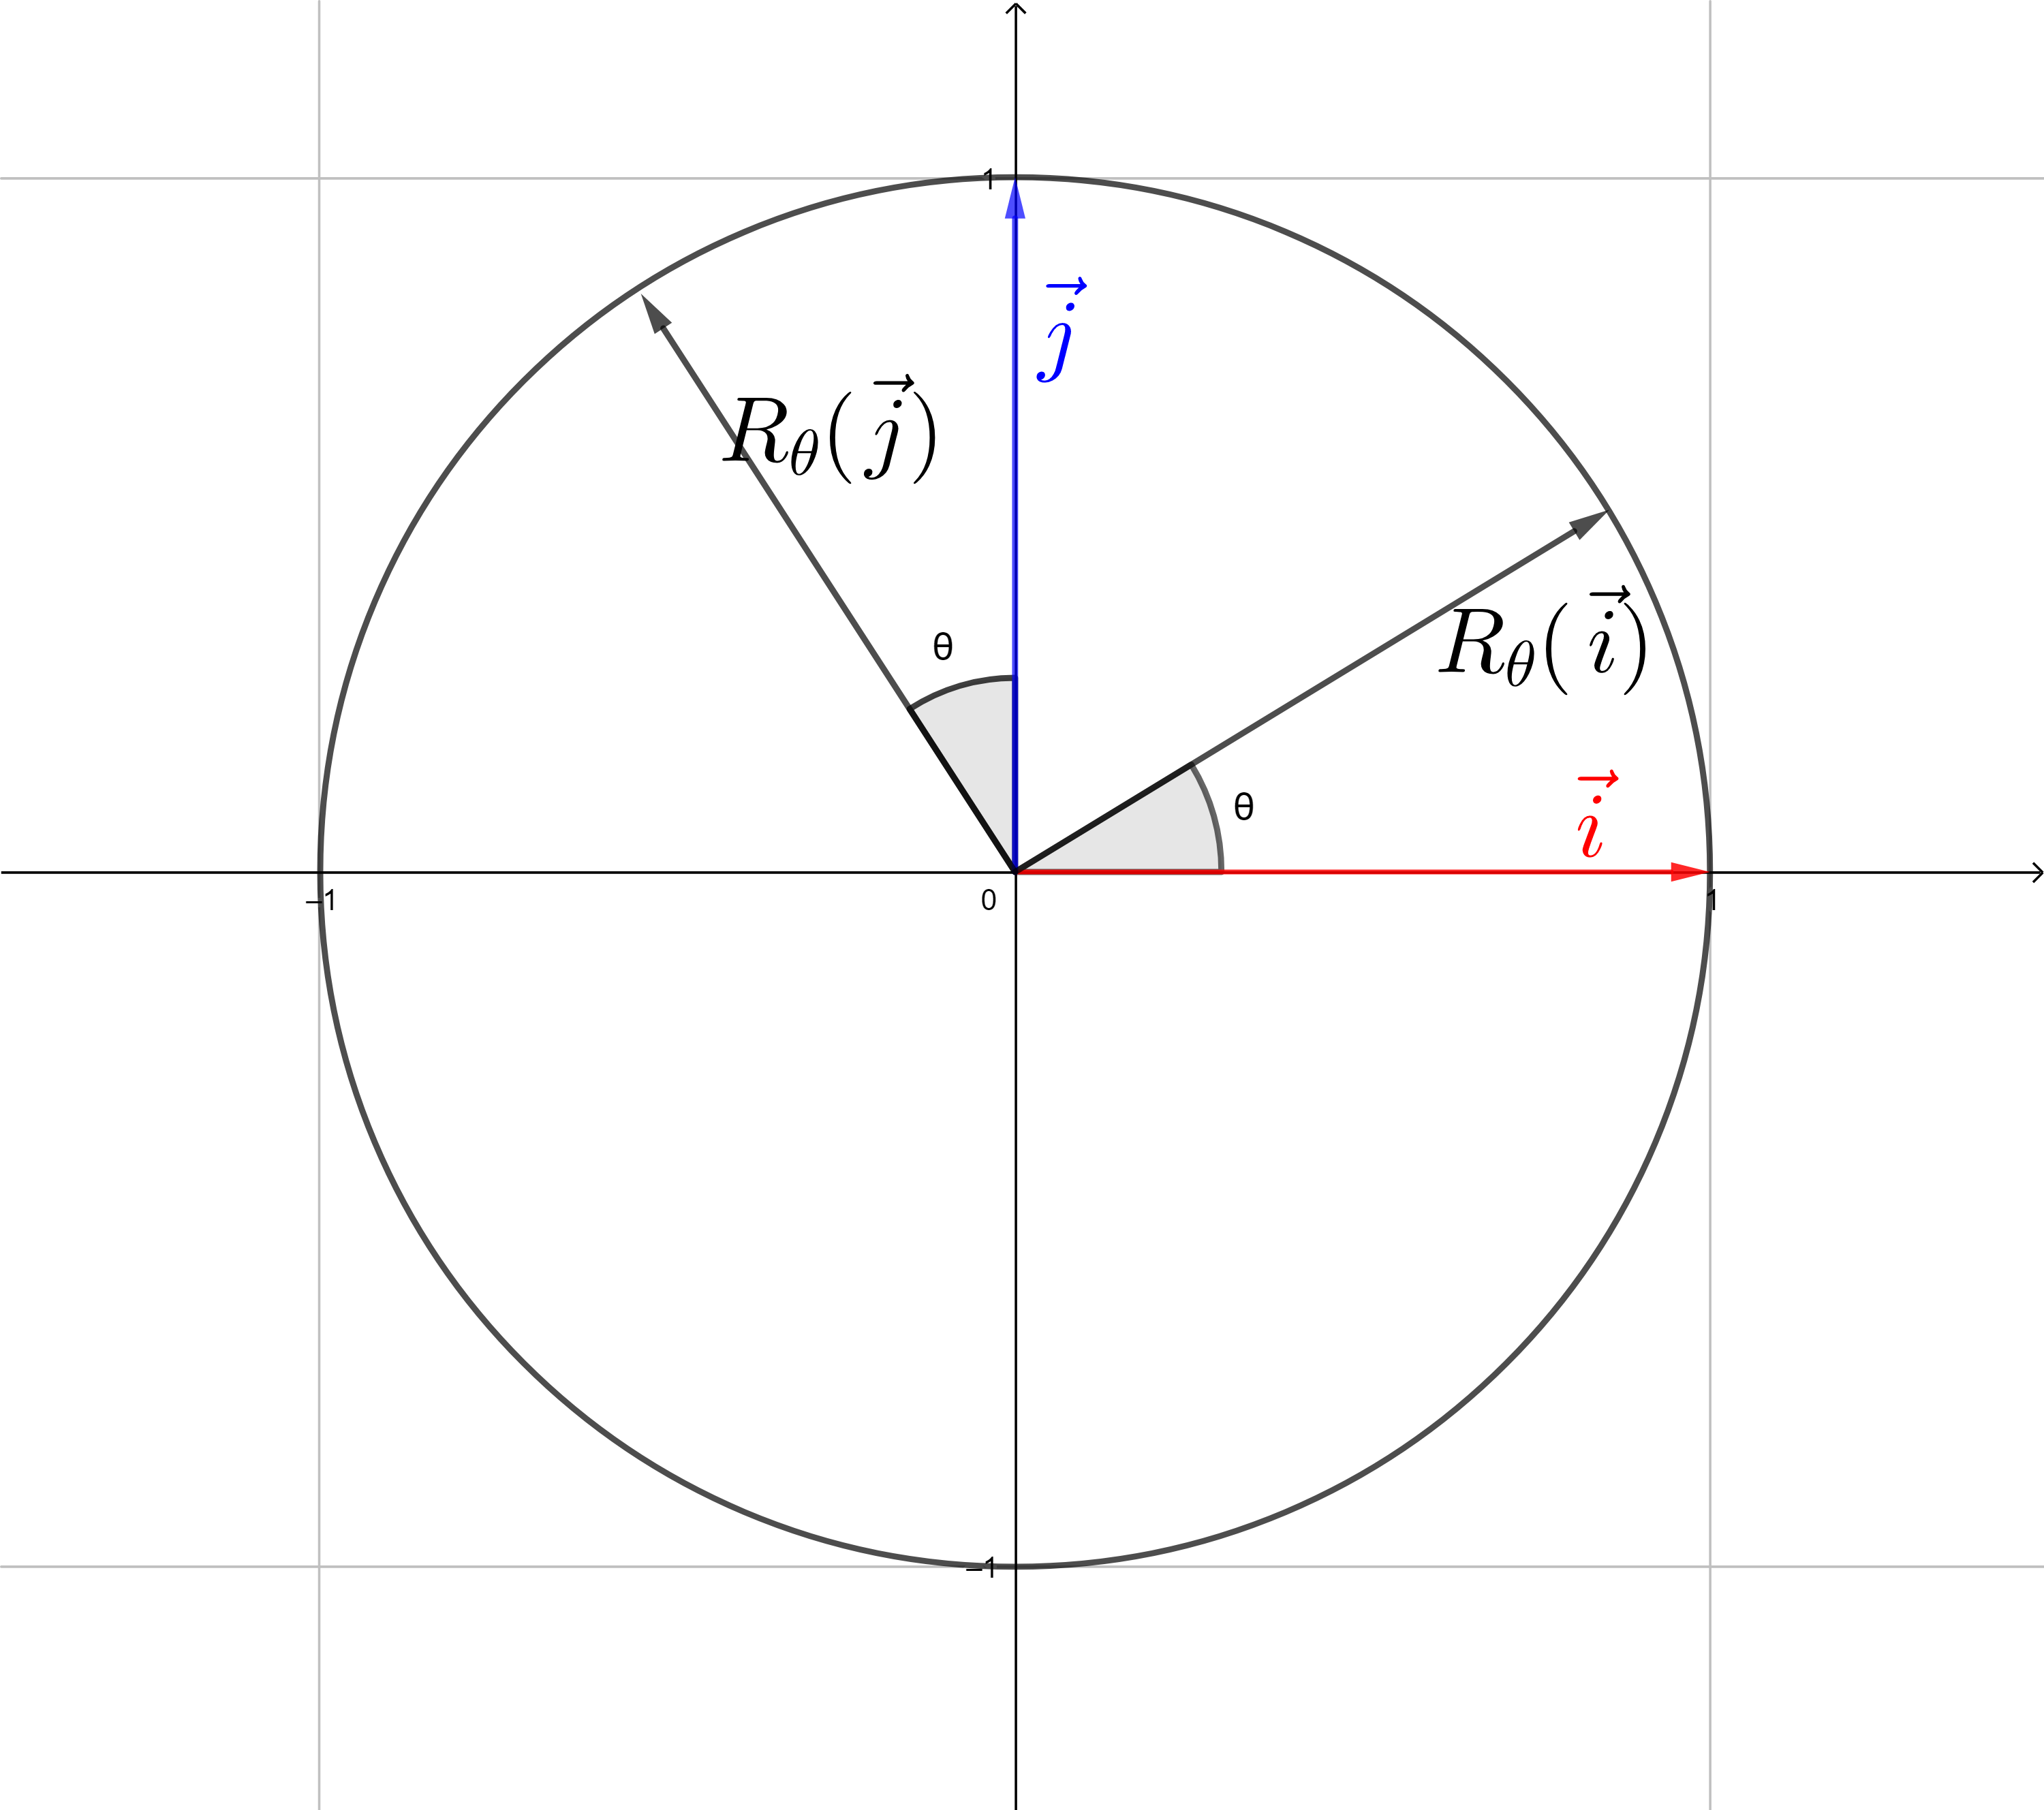
\includegraphics[width=6cm]{rotation.png}
\end{center}
\end{Proposition}
\begin{Demonstration}
Soit $M=\begin{pmatrix}
a &c\\b&d\\
\end{pmatrix}\in\Mn[2]{\R}$. 
$$M\in \mathcal{O}_2(\R) \Leftrightarrow \transposee{M}M=I_2 \Leftrightarrow  \begin{cases}a^2+b^2=1\\ c^2+d^2=1\\ab+cd=0 \end{cases}\Leftrightarrow \exists \theta,\phi\in \R \begin{cases}a=\cos \theta \text{ et }b=\sin \theta\\ c=\cos \phi \text{ et }d=\sin \phi \\\cos \theta \cos \phi +\sin \theta \sin \phi=0 \end{cases}$$
$$
 \Leftrightarrow \exists \theta,\phi\in \R \begin{cases}a=\cos \theta \text{ et }b=\sin \theta\\ c=\cos \phi \text{ et }d=\sin \phi \\\cos (\theta - \phi)=0 \end{cases}
 \Leftrightarrow \exists \theta,\phi\in \R,\exists\epsilon \in\{-1,1\} \begin{cases}a=\cos \theta \text{ et }b=\sin \theta\\ c=\cos \phi \text{ et }d=\sin \phi \\\ \phi=\theta+\epsilon\frac \pi 2[2\pi] \end{cases}$$
 $$
 \overbrace{\Leftrightarrow}^{\cos( \theta+\epsilon\frac \pi 2)=-\epsilon\sin \theta\text{ et }\sin( \theta+\epsilon\frac \pi 2)=\epsilon\cos \theta} \exists \theta\in \R \exists\epsilon \in\{-1,1\}: \quad M=\begin{pmatrix} \cos \theta &-\epsilon\sin \theta \\ \sin \theta & \epsilon \cos \theta \end{pmatrix}
 $$
 On conclut en remarquant que $\det \begin{pmatrix} \cos \theta &-\epsilon\sin \theta \\ \sin \theta & \epsilon \cos \theta \end{pmatrix}=\epsilon$.
\end{Demonstration}
\begin{Proposition}
$R_\theta R_{\theta'}=R_{\theta+\theta'}$ ($\mathcal{SO}_2(\R)$ est un sous-groupe commutatif)et $R_\theta^{-1}= R_{-\theta}$.
\end{Proposition}
\begin{Demonstration}
On a : $$R_\theta R_{\theta'}=\begin{pmatrix} \cos \theta &-\sin \theta \\ \sin \theta & \cos \theta \end{pmatrix} \begin{pmatrix} \cos \theta' &-\sin \theta' \\ \sin \theta' & \cos \theta' \end{pmatrix}=\begin{pmatrix} \cos \theta \cos \theta'- \sin \theta \sin \theta'  &- (\cos\theta \sin \theta'+\sin\theta \cos \theta') \\ \\cos\theta \sin \theta'+\sin\theta \cos \theta' &\cos \theta \cos \theta'- \sin \theta \sin \theta'\end{pmatrix}$$
$$=\begin{pmatrix} \cos(\theta+\theta') &-\sin(\theta+\theta') \\ \sin(\theta+\theta') & \cos(\theta+\theta') \end{pmatrix}=R_{\theta+\theta'}.$$
$R_\theta R_{-\theta}=R_{\theta-\theta}=I_2$ donc $R_\theta^{-1}= R_{-\theta}$.
\end{Demonstration}
On considère $\mathcal{P}$ un plan vectoriel orienté et $\mathcal{B}$ une base orthonormale directe de $\mathcal{P}$.
\begin{Definition}[Rotation]
L'endomorphisme de $\mathcal{P}$ dont la matrice dans $\mathcal{B}$ est $R_{\theta}$ est appelé \defi{rotation d'angle $\theta$} et est noté $r_{\theta}$.
\end{Definition}

\begin{DefinitionProposition}[Angle d'une rotation]
La matrice de $r_{\theta}$ dans toute BOND est $R_{\theta}$.\\
$\theta$ s'appelle \defi{l'angle de la rotation}, il est défini modulo $2\pi$.
\end{DefinitionProposition}
\begin{Demonstration}
Soit $P$ la matrice de passage de la BOND $\mathcal{B}$ à une base BOND $\mathcal{B}'$. Comme $P$ appartient $\mathcal{SO}_2(\R)$, il existe $\theta'$ tel que $P=R_{\theta'}$. La  matrice de $r_{\theta}$ dans la base $\mathcal{B}'$  est : $R_{\theta'}^{-1}R_{\theta}R_{\theta'}=R_{-\theta'}R_{\theta}R_{\theta'}=R_{-\theta'+\theta+\theta'}=R_{\theta}.$
\end{Demonstration}
\begin{Proposition}[Expression complexe d'une rotation]
Soit $r_\theta$ la rotation d'angle $\theta \in \R$. Pour $\vec{x} \in  \mathcal{P}$, on note $z$ l'affixe de $M$ et $z'$ celle de $r_\theta(\vec{x})$.\\
On a :
$$z' = e^{i\theta} z.$$
\end{Proposition}
\begin{Demonstration}
Soit $(x,y)$ les coordonnées du vecteur $\vec{x}$. D'une part, on a :
$$
[r_\theta(\vec{x})]_{\mathcal{B}}=\begin{pmatrix} \cos \theta &-\sin \theta \\ \sin \theta &  \cos \theta \end{pmatrix}=\begin{pmatrix} x&y \end{pmatrix}=\begin{pmatrix}\cos \theta x -\sin \theta y  \\ \sin \theta x + \cos \theta y \end{pmatrix} 
$$
d'autre part, 
$$z' = e^{i\theta} z=e^{i\theta}(x+iy)=(\cos \theta x -\sin \theta y) +i(\sin \theta x + \cos \theta y).$$
On conclut en identifiant la partie réel et imaginaire aux cordonnées de $[r_\theta(\vec{x})]_{\mathcal{B}}$.
\end{Demonstration}
\begin{Definition}[Reflexion]
La \defi{reflexion} d'axe $D$ est la symétrie orthogonal par rapport à $D$. 
\end{Definition}

\begin{Proposition}[Représentation matricielle]
Soit $\mathcal{B}$  une  BOND de $\mathcal{P}$.\\
L'endomorphisme dont la matrice dans $\mathcal{B}$ est $S_\theta = \begin{pmatrix} \cos \theta &\sin \theta \\ \sin \theta &  -\cos \theta \end{pmatrix}$ est la \defi{réflexion} d'axe la droite d'angle polaire $\frac \theta 2$ dans $\mathcal{B}$.
\end{Proposition}
%TODO FAIRE UNE FIGURE ET LA DEMO
\subsection{Isométrie vectorielle dans un espace de dimension 3}
\begin{Theoreme}[Réduction]
Soit $E$ un espace euclidien de dimension $3$ et $u \in \OrE$. Il existe une BOND de $E$ dans
laquelle $u$ a pour matrice :
\begin{enumerate}
\item $\begin{pmatrix}1&0&0\\0& \cos \theta &-\sin \theta \\0& \sin \theta &  \cos \theta \end{pmatrix}$ si $\det u=1$
\item $\begin{pmatrix}-1&0&0\\0& \cos \theta &-\sin \theta \\0& \sin \theta &  \cos \theta \end{pmatrix}$ si $\det u=-1$
\end{enumerate}
avec le cas particulier $\theta = 0 [2\pi]$ :$\begin{pmatrix}-1&0&0\\0& 1 &0 \\0& 0 &  1 \end{pmatrix}$, matrice de réflexion (symétrie orthogonale par rapport à un plan).
\end{Theoreme}
\begin{Demonstration}
Soit $\chi_u$ le polynôme caractéristique de $u$. $\chi_u$ est de degré 3 donc la limite en plus l'infini est de signe opposé à la limite en moins l'infini. D'après  le théorème des valeurs intermédiaires, il existe une racine réelle $\lambda$.\\
Soit $\vec{x}$ un vecteur propre associée à cette valeur propre. par définition, an a  $u(\vec{x})=\lambda\vec{x}$, d'où  $\norme{u(\vec{x})}=|\lambda| \norme{\vec{x}}$. Comme $u$ est une isométrie vectorielle  $\norme{u(\vec{x})}= \norme{\vec{x}}$. Par conséquent $|\lambda|=1$.\\
Considérons le supplémentaire orthogonal de la droite $Vect(\vec{x})$. Ce supplémentaire
est stable sous $u $. En effet soit $\vec{y}$ un élément du supplémentaire. Montrons que $u(\vec{y})\in Vect(\vec{x})^{\perp}.$ 
Soit $\mathcal{B}$ une BON adaptée à $Vect(\vec{x})\oplus Vect(\vec{x})^{\perp}=E.$
On a :
$$[u]_{\mathcal{B}} = \begin{pmatrix}
\pm 1 & 0 &0\\
0 & \cos \theta &-\epsilon\sin \theta \\
0 & \sin \theta & \epsilon\cos \theta
\end{pmatrix}\text{ avec }\epsilon\in\{-1,1\}.$$
Si $\epsilon=1$, on a le premier cas du théorème. 
Si $\epsilon=-1$, la matrice de la restriction de $u$ au sous espace $Vect(\vec{x})^{\perp}$ est une matrice de symétrie orthogonale par rapport à une droite $Vect(\vec{y})$. Soit $\vec{x}$ un vecteur orthogonal à cette droite dans le plan $Vect(\vec{x})^{\perp}$. La matrice de $u$ dans la base $(\vec{x},\vec{y},\vec{z})$ (qui est orthogonale et que nous prenons orthonormée) est donc de la forme
$$[u]_{(\vec{x},\vec{y},\vec{z})} = \begin{pmatrix}
\pm 1 & 0 &0\\
0 & 1 &0 \\
0 & 0 & -1
\end{pmatrix}.$$
qui a permutation des vecteurs de base près est du type voulu.
\end{Demonstration}
\begin{Definition}[Rotation]
        \begin{minipage}[c]{0.45\linewidth}{
La \defi{rotation}, $r_{\vec{x},\theta}$, d'axe $\vec{x}$ et d'angle $\theta$ est l'endomorphisme de $\R^3$ défini par :
\begin{itemize}
\item $r_{\vec{x},\theta}(\vec{x})=\vec{x}$
\item la restriction de 
$f$ au plan $vect \vec{x}^{\perp}$ orienté par
$\vec{x}$ est la rotation (plane) d'angle $\theta$. 
\end{itemize}}
\end{minipage}
    \begin{minipage}[c]{0.45\linewidth}{
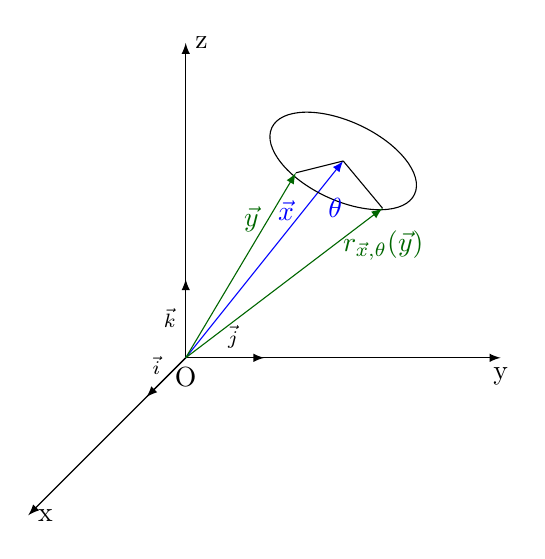
\begin{tikzpicture}
\draw [->,>=latex] (0,0) --++(0,4) node [right] {z};
\draw [->,>=latex] (0,0) --++(-2,-2) node [right] {x};
\draw [->,>=latex] (0,0) --++(4,0) node [below] {y};
\draw [->,>=latex] (0,0) --++(0,1) node [right] {};
\draw [->,>=latex] (0,0) --++(-0.5,-0.5) node [right] {};
\draw [->,>=latex] (0,0) --++(1,0) node [below] {};
\node (O) at (0,0) [below] {O};
\draw [->,>=latex,color=blue] (0,0) -- (2,2.5) node [left,near end] {$ \vec{x}$};
\begin{scope} [shift={(2,2.5)},rotate=-25]
\draw ellipse (1cm and 0.5cm);
\end{scope}
\draw  (2,2.5) -- (2.5,1.9);
\draw  (2,2.5) -- (1.4,2.35);
\draw [->,>=latex,color=green!40!black] (0,0) -- (2.5,1.9) node [right,near end] {$ r_{\vec{x},\theta}( \vec{y}) $};
\draw [->,>=latex,color=green!40!black] (0,0) -- (1.4,2.35) node [left,near end] {$ \vec{y}$};
\node (i) at (-0.2,-0.1) [left] {$\scriptstyle \vec{i}$};
\node (j) at (0.6,0) [above] {$\scriptstyle \vec{j}$};
\node (k) at (0,0.5) [left] {$\scriptstyle \vec{k}$};
\node (k) at (1.9,1.9) [color=blue] {$\theta$}; 
\end{tikzpicture}}
    \end{minipage}
    \end{Definition}

Étude pratique d'une rotation $r$ : détermination du couple axe-angle ($\vec{x},\theta)$.
\begin{enumerate}
\item axe : choisir un vecteur non nul $\vec{x}$ appartenant à $\ker (r-Id_E)$
\item rotation :
\begin{itemize}
\item La trace étant un invariant de similitude, $\tr
r
= 1+2\cos \theta$ ce qui fournit $\cos \theta$
\item la signe de $\sin \theta$ est le même que $\det (\vec{x},\vec{y},r(\vec{y}))$  où
$\vec{y}$ est un vecteur non colinéaire à $\vec{x}$.  En
effet : $\det (\vec{x},\vec{y},r(\vec{y})) =\det \begin{pmatrix}
1 & x_1& x_1\\
0 & x_2 & x_2\cos \theta - x_3\sin \theta\\
0 & x_3 &  x_2\sin \theta + x_3\cos \theta
\end{pmatrix}=(x_2^2+x_3^2)\sin \theta.$ 
\end{itemize} 
\end{enumerate}
\begin{Exemple}
Caractériser l'endomorphisme $f$ de $\R^3$ dont la matrice dans la base canonique est
$$A= \frac 1 3 \begin{pmatrix}
2&-1&2\\
2&2&-1\\
-1&2&2
\end{pmatrix}.$$
\begin{itemize}
\item rotation vectoriel : les colonnes de $A$ forment une base orthonormée donc $f$ endomorphisme orthogonal. De plus  $\det(A)=1$, $f$ est  une rotation.
\item axe :  on obtient $\Ker(A-I_3)=Vect(1,1,1).$ Posons $\vec{x}=(1,1,1)$. 
\item angle :
\begin{itemize}
\item  $\tr(A)=2$, et donc $\cos \theta =\frac 1 2$, soit $\theta=\pm \frac \pi 3[2\pi]$. Pour déterminer le signe de $\theta$, on pose $\vec{y}=(1,-1,0)$ non colinéaire  $\vec{x}$. $f(\vec{y})=(1,0,-1)$ et $\det (\vec{x},\vec{y},r(\vec{y}))=3>0$. ce qui signifie $\theta\theta\in]0,\pi[ modulo 2\pi.$ On en déduit donc que $f$ est la rotation d'axe dirigé par $(1,1,1)$ et d'angle $\frac \pi 3$.
\end{itemize}
\end{itemize}
\end{Exemple}



%% -----------------------------------------------------------------------------
\section{Endomorphismes symétriques et Matrices symétriques}
\subsection{Généralités}
\begin{Definition}[Endomorphismes symétriques]
Soit $u\in \LE$.\\
On dit que $u$ est un endomorphisme \defi{symétrique} (ou \emph{autoadjoint}) si 
$$\forall \vec{x},\vec{y}\in E:\quad \PS{u(\vec{x})}{\vec{y}} = \PS{\vec{x}}{u(\vec{y})}.$$
On note $\SE$ l'ensemble des endomorphismes symétriques de $E$.\\
Il s'agit d'un sous-espace vectoriel de $\LE$.
\end{Definition}
\begin{Definition}[Matrices symétriques]
Une matrice \defi{symétrique}, $S$, est une matrice carrée qui est égale à sa propre transposée, soit $\transposee{S}=S$.\\
On note $\SnR$ est l'ensemble des matrices symétriques de taille $n$.\\
Il s'agit d'un sous-espace vectoriel de $\Mn{n}{\R}$ et $\dim \SnR=  \frac{n(n+1)}{2}$.
\end{Definition}



\begin{Exemple}La matrice suivante est  symétrique :
$$\begin{pmatrix}2&4&6\\4&0&10\\6&10&12\end{pmatrix}$$
Toute matrice diagonale est symétrique.\\
Soit $X\in \R^n$. Alors $X  \transposee{X}$ est symétrique.\\
Soit $A\in \Mn{n}{\R}$. Alors $\transposee{A} A$ est symétrique.\\
\end{Exemple}
\begin{Exemple}[Matrice hessienne]
Soit $f$ une fonction de classe $\mathcal {C}^{2}(\mathbb{R}^2,\mathbb{R})$. Sa matrice hessienne $$\begin{pmatrix}\frac {\partial ^{2}f}{\partial x_{1}^{2}}&\frac {\partial ^{2}f}{\partial x_{1}\partial x_{2}}\\\frac {\partial ^{2}f}{\partial x_{2}\partial x_{1}}&\frac {\partial ^{2}f}{\partial x_{2}^{2}}\end{pmatrix}$$ est symétrique.
\end{Exemple}

\begin{Exemple}[Matrice de covariance]La matrice de covariance du vecteur aléatoire $\vec {X}=\begin{pmatrix}X_{1}\\X_{2}\end{pmatrix}$ définie par:
$$\operatorname {Var} ({\vec {X}})={\begin{pmatrix}\operatorname {Var} (X_{1})&\operatorname {Cov} (X_{1},X_{2})\\\operatorname {Cov} (X_{2},X_{1}) &  \operatorname {Var} (X_{2}) \end{pmatrix}}$$ est symétrique.
\end{Exemple}
\begin{Proposition}[Endomorphisme symétrique et matrice symétrique]
Soit $u\in \LE$.\\
Les conditions suivantes sont équivalentes:
\begin{enumerate}[label=\roman*.]
\item $u$ est un endomorphisme symétrique;
\item pour toute base orthonormale $\mathcal{B}$ de $E$,
  $[u]_\mathcal{B}$ est une matrice symétrique;
\item il existe une base orthonormale $\mathcal{B}$ de $E$
  telle que $[u]_\mathcal{B}$ est une matrice symétrique.
\end{enumerate}
\end{Proposition}
\begin{Proposition} Muni du produit scalaire canonique sur $\R^n$,  une matrice $S$ est symétrique si et seulement si :
$$\forall X,Y\in  \R^n, \quad  \PS{SX}{Y}=\PS{X}{SY}.$$
\end{Proposition}
\begin{Definition}[Matrices antisymétriques]
Une matrice \defi{antisymétrique}, $A$, est une matrice carrée qui est égale à l'opposée de sa propre transposée, soit $\transposee{A}=-A$.\\
On note $\AnR$ est l'ensemble des matrices antisymétriques de taille $n$.\\
Il s'agit d'un sous-espace vectoriel de $\Mn{n}{\R}$ et $\dim \AnR=  \frac{n(n-1)}{2}$.
\end{Definition}
\begin{Proposition}[Supplémentaires orthogonaux]
$\AnR$ et $SnR$ sont des supplémentaires orthogonaux par rapport au produit scalaire  $(A,B)\mapsto \tr(\transposee{A}B)$.\\
La décomposition d'une matrice $M$ selon cette somme directe est : 
$$M= \frac{M+\transposee{M}}{2}+ \frac{M-\transposee{M}}{2}.$$
\end{Proposition}

\subsection{Produit scalaire}
\begin{Definition}[Positive]
Une matrice symétrique, $S$, est \defi{positive} si $$\forall X\in  \R^n :\quad \transposee X S X \geq 0.$$
\end{Definition}
\begin{Definition}[Définie]
Une matrice symétrique, $S$, est \defi{définie} si $$\forall X\in \R^n :\quad \transposee X S X = 0 \Rightarrow X = 0.$$
\end{Definition}
\begin{Proposition}[Produit scalaire associée à une matrice symétrique positive et définie]
Soit $S$ une matrice symétrique, définie et positive.\\
Alors $\Fonction{\PS{}{}}{\R^n\times \R^n }{\mathbb{R}}{(X,Y)}{\transposee{X} S Y}$ est un produit scalaire.
\end{Proposition}
\begin{Proposition}[Expression d'une produit scalaire associée à l'aide une matrice symétrique positive et définie]
Soit $(E,\PS{.}{.})$ un espace euclidien. Soit $\mathcal{B}=(\vec{e}_1,\dots,\vec{e}_n)$ une base quelconque de $E$.\\
Alors
$$\forall \vec{x},\vec{y}\in E, \PS{\vec{x}}{\vec{y}}=\transposee{[\vec{x}]_{\mathcal{B}}}\times S \times [\vec{y}]_{\mathcal{B}} \text{ avec } S=\begin{pmatrix}\PS{\vec{e}_1}{\vec{e}_1}&\PS{\vec{e}_1}{\vec{e}_2}&\cdots &\PS{\vec{e}_1}{\vec{e}_n}\\ \PS{\vec{e}_2}{\vec{e}_1}&\PS{\vec{e}_2}{\vec{e}_2}&\cdots &\PS{\vec{e}_2}{\vec{e}_n}\\\vdots &\vdots &\ddots &\vdots \\\PS{\vec{e}_n}{\vec{e}_1}&\PS{\vec{e}_n}{\vec{e}_2}&\cdots &\PS{\vec{e}_n}{\vec{e}_n}\end{pmatrix}.$$
Ainsi définie, $S$ est une matrice symétrique définie et positive. 
\end{Proposition}


\subsection{Diagonalisation}

\begin{Lemme}[Stabilité et orthogonal]
Soit $u$ un endomorphisme symétrique de $E$. Soit $F$ sous espace vectoriel stable par
$u$.\\
Alors son orthogonal $F^{\perp}$ est également stable par $u$.
\end{Lemme}

\begin{Lemme}[Sous espace propres orthogonaux]
Soit $u$ un endomorphisme symétrique de $E$.\\
Alors les sous-espaces propres de $S$ sont deux à deux orthogonaux.
\end{Lemme}

\begin{Theoreme}[Théorème spectral (endomorphisme symétrique)]
Tout endomorphisme symétrique est diagonalisable dans une base orthonormale et ses valeurs propres sont toutes réelles.
\end{Theoreme}
\begin{Demonstration}
Soit $u$ un endomorphisme symétrique et \\
On montre d'abord qu'il  existe au moins une valeur propre réelle, puis on restreint $u$ par récurrence sur la dimension de l'espace :
\begin{itemize}
\item Tant que $u$ est un endomorphisme  de dimension non nulle 
\begin{itemize}
\item Existence d'une valeur propre réel : soit $S$ la matrice de $u$ dans une base quelconque. Il existe $\lambda$ une racine a priori complexe de son polynôme caractéristique et $X$ un vecteur propre complexe non nulle telle que $AX=\lambda X$.\\
Alors
$$ \begin{cases} \transposee{(SX)}\overline{X}=\lambda \transposee{X}\overline{X}\\
\transposee{(SX)}\overline{X}=\transposee{X}\transposee{S}\overline{X}=\transposee{X}S\overline{X}=\transposee{X}\overline{SX}=\transposee{X}\overline{\lambda X}=\overline{\lambda}\transposee{X}\overline{X} \\
\end{cases} $$
Comme  $\transposee{X}\overline{X}\neq 0$, $\lambda=\overline{\lambda}$, donc $\lambda$ est réel.
\item Soit $E_\lambda$ l'espace propre associée à la valeur propre $\lambda$. On a $E_\lambda\oplus E^{\perp}_\lambda=E$. D'après le lemme,   $E^{\perp}_\lambda$ est stable par $u$. Alors $u$ devient la restriction de $u$ à $E^{\perp}_\lambda$.
\end{itemize}
\end{itemize}


\end{Demonstration}
\begin{Theoreme}[Théorème spectral (matrice symétrique)]
Soit $S$ une matrice symétrique réelle.\\
Alors il existe une matrice $P$ orthogonale  et une matrice $D$ diagonale dont tous les coefficients sont réels, telles que la matrice A est égale à $PDP^{-1}=PD\transposee{P}$.
\end{Theoreme}



\begin{Proposition}[Caractérisation de la projection orthogonale]
Soit $p \in \LE$ un projecteur et $s$ une symétrie.\\
 Alors $p$ est une projection orthogonale si et seulement si $p$ est un endomorphisme symétrique.\\
  Alors $s$ est une symétrie orthogonale si et seulement si $s$ est un endomorphisme symétrique.
\end{Proposition}



\end{document}
